\section{Les revues de presse}
\label{sec:revue}

La principale fonctionnalité innovante de notre plateforme de consultation de journaux anciens est la possibilité de créer et de partager des revues de presse.

Une revue de presse, ou parcours thématique, est une liste d'articles de journaux regroupés ensemble par un ou plusieurs utilisateurs autour d'une thématique précise, comme par exemple une date, un événement ou une zone géographique.

La création d'une revue de presse se fera de deux façons différentes, d'abord depuis le menu principal, il y aura un bouton permettant de créer une revue de presse vide. L'autre méthode consiste à cliquer sur le bouton d'ajout présent sur la page de consultation et de cliquer sur le-dit bouton pour créer une nouvelle revue de presse. La seule différence avec la première méthode est que la revue de presse sera initialisée avec le-dit document.

La page de visualisation d'une revue de presse sera composée du titre, de la description de la revue de presse et d'une liste comprenant les articles de celle-ci. Depuis cette page il sera possible de modifier le titre, la description et de retirer un article sur cette revue de presse. L'auteur pourra également modifier l'ordre de lecture des articles en glissant l'article à la position souhaitée.

\begin{figure}[H]
    \centering
    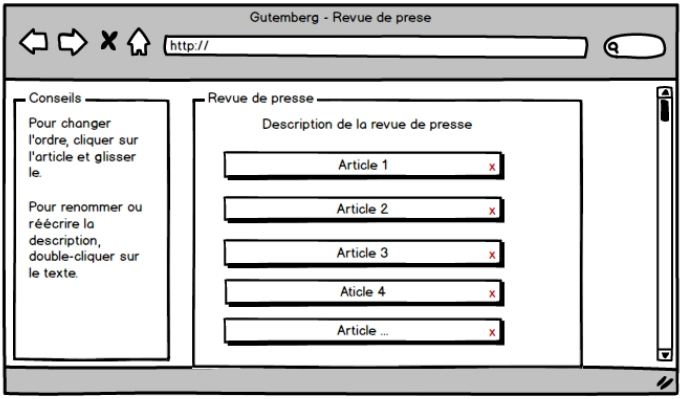
\includegraphics[width=\textwidth]{figures/revue.png}
    \caption{Page de visualisation d'une revue de presse}
    \label{fig:revue}
\end{figure}

